\chapter{Valuation Multiples}\label{ch:multiples}

\emph{Based on Lecture L11 (file ``L10 -- Multiples'', 32 slides): ``Valuation Multiples'', 2--3 November 2026, and on the official solution file \texttt{Bridge\_SOL.xlsx} (Equity Value vs Enterprise Value). Workflow step: \textbf{multiples} and \textbf{value bridge}.}

\section{Plan for the Day}
\textbf{Last time}: FCFE discount models; differences between DDM and FCFE (Chapter~\ref{ch:fcfe}).\\
\textbf{Today}: the principles of relative valuation; the basic steps for using common multiples.\\
\textbf{Agenda}: (1) use of relative valuation: overview, principles, why; (2) using multiples: metrics, steps, deal multiples; (3) common multiples: P/E, P/BV, EV/EBITDA, EV/Sales.

% =====================================================================
\section{Use of Relative Valuation}

\subsection{Overview (Reminder)}
\begin{center}
\begin{tikzpicture}[m/.style={fill=navy!75,text=white,rounded corners=3pt,minimum width=2.6cm,minimum height=0.9cm,font=\bfseries},
  d/.style={fill=navy!15,rounded corners=3pt,text width=6.4cm,minimum height=0.9cm,font=\small,align=center}]
\node[m] (M) at (0,0) {Methods};
\node[m] (I) at (4,1.6) {Intrinsic}; \node[d] at (9.2,1.6) {Explicit forecast of cash flows, discounted at the appropriate cost of capital};
\node[m,fill=gray!30,text=black] (X) at (4,0) {Mix}; \node[d,fill=gray!10] at (9.2,0) {Value early cash flows explicitly with an absolute method, then apply a multiple};
\node[m] (R) at (4,-1.6) {Relative}; \node[d] at (9.2,-1.6) {Multiply the relevant variables of your firm (EPS, FCFO, \dots) by multiples observed in the market};
\foreach \x in {I,X,R} \draw[thick,navy!50] (M.east) -- (\x.west);
\end{tikzpicture}
\end{center}
\begin{addbox}
The ``mix'' is exactly the DCF with a TV computed from a multiple (Chapter~\ref{ch:growth}): if the multiple comes from comparables, the TV turns the DCF into a partly relative valuation.
\end{addbox}

\subsection{Principles}
In a relative valuation, the value of an asset is compared to the values the market assesses for \textbf{comparable} assets. Two basic components:
\begin{enumerate}
  \item \textbf{Standardized prices}: prices are converted into multiples of earnings (P/E), BV (P/BV), sales (EV/Sales), etc., so that they are \textbf{independent of size}.
  \item \textbf{Similar or comparable firms} (peers): \textbf{no two firms are identical}, and firms in the same business can still differ in risk, growth and cash flows.
\end{enumerate}
Multiples can be sourced from two markets:
\begin{itemize}
  \item \textbf{Stock market (market or trading multiples)}: stand-alone values (no acquisition premiums or minority discounts embedded);
  \item \textbf{M\&A market (deal or transaction multiples)}: prices paid in M\&A deals (acquisition premiums or minority discounts embedded).
\end{itemize}
\begin{keybox}
Ignoring speculative phenomena (bubbles, \dots), the difference between market and deal multiples is explained by \textbf{acquisition premiums} or \textbf{minority discounts}.
\end{keybox}

\subsubsection*{Numerator and denominator}
\begin{center}
\begin{tikzpicture}[t/.style={draw,rounded corners=5pt,align=left,font=\scriptsize,inner sep=4pt},b/.style={draw,align=left,font=\scriptsize,inner sep=3pt,text width=3.1cm,minimum height=2.3cm,anchor=north}]
\node[t] (n1) at (-5,2.3) {Market value of equity};
\node[t] (n2) at (-0.6,2.3) {Market value of the firm\\Firm value $=$ MV equity $+$ MV debt};
\node[t] (n3) at (4.6,2.3) {Market value of operating assets\\Enterprise value (EV) $=$ MV equity\\\quad$+$ MV debt $-$ Cash};
\node[font=\small] at (0,0.9) {Multiple $=\dfrac{\text{Numerator}=\text{What you are paying for the asset}}{\text{Denominator}=\text{What you are getting in return}}$};
\node[b] at (-5.4,-0.2) {\textbf{Revenues}\\a.\ Accounting revenues\\b.\ Drivers: \# customers, \# subscribers, \# units};
\node[b] at (-1.8,-0.2) {\textbf{Earnings}\\a.\ To equity investors: net income, EPS\\b.\ To firm: operating income (EBIT)};
\node[b] at (1.8,-0.2) {\textbf{Cash flow}\\a.\ To equity: NI $+$ depreciation; FCFE\\b.\ To firm: EBIT $+$ D\&A (EBITDA); FCFF};
\node[b] at (5.4,-0.2) {\textbf{Book value}\\a.\ Equity $=$ BV equity\\b.\ Firm $=$ BV debt $+$ BV equity\\c.\ Invested capital $=$ BV equity $+$ BV debt $-$ cash};
\end{tikzpicture}
\end{center}
\begin{addbox}[Consistency rule]
Numerator and denominator must refer to the \textbf{same claimholders}: equity value with equity measures (net income, EPS, BV of equity, FCFE); EV with firm measures (revenues, EBITDA, EBIT, FCFF, invested capital). Mixing them (e.g., P/Sales or EV/Net income) is inconsistent, and the slide on revenue multiples calls P/S ``inconsistent'' for this reason.
\end{addbox}

\subsubsection*{From EV to equity value: the bridge-to-equity}
\begin{center}
\begin{tikzpicture}[font=\small]
\node[font=\small\bfseries,text=navy] at (-5.6,4.4) {Market values}; \node[font=\small\bfseries] at (0,4.4) {Book values}; \node[font=\small\bfseries,text=navy] at (5.6,4.4) {Market values};
\draw (-3.6,3.9) rectangle (0,3.1); \node[font=\scriptsize\bfseries] at (-1.8,3.5) {Noncash nondebt WC};
\draw (-3.6,3.1) rectangle (0,2.3); \node[font=\scriptsize\bfseries] at (-1.8,2.7) {Fixed assets};
\draw (-3.6,2.3) rectangle (0,0.8); \node[font=\scriptsize,align=left] at (-1.8,1.55) {\textbf{Surplus items:}\\$+$ Associates\\$-$ Pension deficit\\$\pm$ Others};
\draw (0,3.9) rectangle (3.6,2.8); \node[font=\scriptsize,align=left] at (1.8,3.35) {\textbf{Net debt:}\\$+$ Financial debt\\$-$ Cash \& equivalents};
\draw (0,2.8) rectangle (3.6,2.0); \node[font=\scriptsize\bfseries] at (1.8,2.4) {Group's equity};
\draw (0,2.0) rectangle (3.6,1.4); \node[font=\scriptsize\bfseries] at (1.8,1.7) {Minorities (NCI)};
\draw (0,1.4) rectangle (3.6,0.8); \node[font=\scriptsize\bfseries] at (1.8,1.1) {Preferred E};
\draw[decorate,decoration={brace,amplitude=4pt,mirror}] (-3.7,3.9) -- (-3.7,2.3) node[midway,left=5pt,font=\small\bfseries,text=navy] {EV};
\draw[decorate,decoration={brace,amplitude=4pt}] (3.7,2.8) -- (3.7,2.0) node[midway,right=5pt,font=\small\bfseries,text=navy] {EqV};
\end{tikzpicture}

\medskip
\begin{tikzpicture}[b/.style={fill=navy,text=white,font=\scriptsize\bfseries,minimum width=1.2cm,minimum height=0.8cm,align=center}]
\foreach \i/\t/\s in {0/EV/{$-$},1/{Net\\debt}/{$+$},2/{Assoc.}/{$-$},3/{Pension\\deficit}/{$-$},4/NCI/{$-$},5/{Preferred\\shares}/{$\pm$},6/{Surplus\\items}/{$=$}}{
  \node[b] at (1.75*\i,0) {\t}; \node at (1.75*\i+0.875,0) {\s};}
\node[b] at (12.25,0) {EqV};
\end{tikzpicture}
\end{center}
\[
\text{EqV}=\text{EV}-\text{Net debt}+\text{Associates}-\text{Pension deficit}-\text{NCI}-\text{Preferred shares}\pm\text{Surplus items}
\]
\begin{addbox}
This is the same bridge as Chapter~\ref{ch:fcf} (there with the tax adjustment on pension and debt-like provisions). EV refers to the operating business only, so all non-operating assets are added and all non-common-equity claims are subtracted.
\end{addbox}

\subsection{Official Exercise: Equity Value vs Enterprise Value (Bridge\_SOL Excel)}

\begin{exbox}[Firm A: from equity value to EV (\euro m, except per share)]
Share price \euro18.76; basic shares 1,342.7m; diluted shares 1,351.6m. LTM revenue 11,858; LTM EBITDA 2,099; LTM net income 755.
\begin{center}
\small
\begin{tabular}{@{}lr@{}}
\toprule
Diluted equity value ($1{,}351.6\times18.76$) & 25,356.0\\
$-$ Cash \& cash equivalents & (868)\\
$-$ Equity investments & (290)\\
$-$ Other non-core assets, net & (17,983)\\
$+$ Total debt & 12,243\\
$+$ Preferred stock & 0\\
$+$ Noncontrolling interests & 1,659\\
$+$ Unfunded pension obligations & 674\\
$+$ Restructuring \& legal liabilities & 2,849\\
\midrule
\textbf{Enterprise value} & \textbf{23,640.0}\\
\bottomrule
\end{tabular}
\end{center}
LTM EV/Revenue $=23{,}640/11{,}858=\mathbf{1.99\times}$; LTM EV/EBITDA $=23{,}640/2{,}099=\mathbf{11.26\times}$; LTM P/E $=25{,}356/755=\mathbf{33.58\times}$.
\end{exbox}

\begin{exbox}[What happens to EqV, EV and the multiples after each transaction of \euro1,000? (official Excel)]
\small
\begin{tabular}{@{}lrrrrrrr@{}}
\toprule
Transaction & $\Delta$Cash & $\Delta$Debt & $\Delta$Equity & $\Delta$Pref. & \textbf{EqV} & \textbf{EV} & \textbf{P/E}\\
\midrule
Base case & -- & -- & -- & -- & 25,356 & 23,640 & 33.58$\times$\\
Issue \euro1,000 of shares & $+1{,}000$ & 0 & $+1{,}000$ & 0 & 26,356 & 23,640 & 34.91$\times$\\
Raise \euro1,000 of debt & $+1{,}000$ & $+1{,}000$ & 0 & 0 & 25,356 & 23,640 & 33.58$\times$\\
Repurchase \euro1,000 of shares & $-1{,}000$ & 0 & $-1{,}000$ & 0 & 24,356 & 23,640 & 32.26$\times$\\
Repay \euro1,000 of debt & $-1{,}000$ & $-1{,}000$ & 0 & 0 & 25,356 & 23,640 & 33.58$\times$\\
Pay \euro1,000 of dividends & $-1{,}000$ & 0 & $-1{,}000$ & 0 & 24,356 & 23,640 & 32.26$\times$\\
Issue \euro1,000 of preferred & $+1{,}000$ & 0 & 0 & $+1{,}000$ & 25,356 & 23,640 & 33.58$\times$\\
\bottomrule
\end{tabular}

\medskip
EV/Revenue (1.99$\times$) and EV/EBITDA (11.26$\times$) are \textbf{unchanged in every case}. Example (issue shares): EqV $25{,}356+1{,}000=26{,}356$; cash $-868-1{,}000=-1{,}868$; EV $=26{,}356-1{,}868-290-17{,}983+12{,}243+1{,}659+674+2{,}849=23{,}640$.
\end{exbox}
\begin{keybox}[Key point of the exercise (official Excel)]
No matter how a company is financed, its \textbf{enterprise value stays the same}. Equity value may change depending on the mix of equity, debt, cash and preferred stock. As a result, \textbf{EV-based multiples do not change} when financing changes (at least immediately after the change). In real life EV \emph{is} affected by capital structure, because WACC changes with financing (Chapter~\ref{ch:capstr}), but EV still changes by \textbf{far less} than equity value.
\end{keybox}
\begin{addbox}[Reading the table]
Equity value changes only when cash flows between the firm and its \emph{shareholders} (share issue, buyback, dividend). Debt and preferred transactions swap cash for a claim of equal amount, so EqV is unchanged; EV never moves because cash and the claim offset in the bridge. P/E therefore moves with buybacks and dividends, but EV/EBITDA does not. In the Excel, pension and restructuring liabilities are added without the $(1-t)$ adjustment of Chapter~\ref{ch:fcf}: in an exam, follow the data given.
\end{addbox}

\subsection{Why Relative Valuation?}
Reasons why relative valuations are widely used:
\begin{enumerate}
  \item \textbf{Few explicit assumptions}: far fewer explicit assumptions and far quicker than DCF valuations.
  \item \textbf{Market-oriented}: more likely to reflect the current \textbf{market mood}, since they measure relative (not intrinsic) value.
  \item \textbf{Simplicity}: simpler to understand and easier to present (easier to frame an asset as cheap or expensive).
\end{enumerate}
Most valuations on Wall Street are relative: almost all equity reports and almost all acquisition valuations are based on multiples and comparables; rules of thumb based on multiples are common and often the basis for final judgments.

\textbf{The strengths are also the major weaknesses}:
\begin{enumerate}
  \item \textbf{Few explicit assumptions}: the ease of relative valuation can produce \textbf{inconsistent estimates} where key variables (risk, growth, cash flows) are ignored.
  \item \textbf{Market oriented}: values are too high/low when the market is \textbf{over/undervaluing comparables}.
  \item \textbf{Simplicity (bias)}: the \textbf{lack of transparency} on underlying assumptions makes multiples vulnerable to manipulation.
\end{enumerate}

% =====================================================================
\section{Using Multiples}

\subsection{Metrics: Time Frame}
Suppose it is 30/9/2026. The denominator can be:
\begin{itemize}
  \item \textbf{Actual}: last fiscal year (LFY, 31/12/2025);
  \item \textbf{Forward}: next FY (2026) or following years (2027, \dots);
  \item \textbf{Trailing}: last four quarters (LTM): Q4 2025 $+$ Q1/Q2/Q3 2026 (the slide writes ``Q4 2015'', a typo).
\end{itemize}
Choice: \textbf{LFY/LTM} if no estimates exist (for comparables or target); \textbf{F+1, F+2, \dots} if LFY/LTM figures are negative and/or for growing or innovative businesses. Business plans usually forecast growth: EBITDA 27E $>$ EBITDA 26A $\Rightarrow$ \textbf{forward multiple $<$ actual multiple}.
\begin{keybox}
\textbf{The numerator never changes!} Future EV and EqV do not exist: the numerator is always today's market value.
\end{keybox}

\begin{exbox}[Slide question: forward (T+1) EBITDA multiple -- target's EqV at end-2025]
\begin{center}
\small
\begin{tabular}{@{}lrrr@{}}
\toprule
& 2025 & 2026 & 2027\\
\midrule
\multicolumn{4}{@{}l}{\emph{Peer company}}\\
Market cap & 1,000 & & \\
EBITDA & 100 & 120 & 150\\
Net debt & 200 & 205 & 215\\
\multicolumn{4}{@{}l}{\emph{Target company}}\\
Equity value & ? & & \\
EBITDA & 20 & 25 & 30\\
Net debt & 10 & 15 & 20\\
\bottomrule
\end{tabular}
\end{center}
Options on the slide: 241; 235; 240; 236. \emph{Solution} -- \checkmark\ \textbf{confirmed by the official class solution} (Multiples\_SOL.xlsx, sheet Ex\_1: EV peer 1,200; EV/EBITDA 10.0$\times$; EV target 250; EqV target \textbf{240}):
\begin{align*}
\text{Peer EV (today)}&=1{,}000+200=1{,}200\qquad\text{EV/EBITDA}_{26}=1{,}200/120=10.0\times\\
\text{Target EV}&=10.0\times25=250\qquad\text{Target EqV}=250-10\ (\text{today's net debt})=\mathbf{240}
\end{align*}
The wrong options come from using a future net debt: peer net debt 205 gives $1{,}205/120\times25-10=\mathbf{241}$ or $-15=\mathbf{236}$; target net debt 15 gives $250-15=\mathbf{235}$. Only the denominator moves forward; EV and net debt are today's.
\end{exbox}

\begin{exbox}[Consistency between peers and target (slide)]
\begin{center}
\small
\begin{tabular}{@{}lrrrrr@{}}
\toprule
& Mkt cap & NI 25A & NI 26E & P/E actual & P/E FWD\\
\midrule
Peers & 10,000 & 550 & 605 & $10{,}000/550=18.2\times$ & $10{,}000/605=16.5\times$\\
Target & & 190 & 240 & & \\
\bottomrule
\end{tabular}
\end{center}
Equity value as of end-2025:
\begin{itemize}[leftmargin=*]
  \item with P/E actual: $190\times18.2=\mathbf{3{,}455}$ \checkmark
  \item with P/E FWD: $240\times16.5=\mathbf{3{,}967}$ \checkmark
  \item \textcolor{keyred}{incorrect}: $190\times16.5=3{,}140$ (actual earnings $\times$ forward multiple)
  \item \textcolor{keyred}{incorrect}: $240\times18.2=4{,}364$ (forward earnings $\times$ actual multiple)
\end{itemize}
\end{exbox}

\subsection{Metrics: Calendarization}
Assume the target's FY ends on 31/12 and the peers' FY ends on 31/3: the peers' figures must be \textbf{calendarized} as of 31/12.
\begin{center}
\begin{tikzpicture}[x=1.25cm,font=\scriptsize]
\foreach \x/\l in {0/{1/1/25},1/{3/31/25},2/{6/30/25},3/{9/30/25},4/{12/31/25},5/{3/31/26},6/{6/30/26},7/{9/30/26},8/{12/31/26},9/{3/31/27}}{\draw[dashed,gray] (\x,0.3) -- (\x,-3.6); \node[font=\tiny\bfseries] at (\x,0.55) {\l};}
\draw[very thick,navy] (0,0) -- (3.95,0) node[pos=0.5,below,font=\scriptsize\bfseries] {Target FY 25: A};
\draw[very thick,navy] (4.05,0) -- (8,0) node[pos=0.5,below,font=\scriptsize\bfseries] {Target FY 26: B};
\draw[very thick,gray] (1,-1) -- (4.95,-1) node[midway,below] {Peers FY 25: C};
\draw[very thick,gray] (5.05,-1) -- (9,-1) node[midway,below] {Peers FY 26: D};
\foreach \a/\b/\l in {4/5/Q4 of C,5/6/Q1 of D,6/7/Q2 of D,7/8/Q3 of D}{\draw[thick,gray] (\a+0.05,-2) -- (\b-0.05,-2); \node at ({(\a+\b)/2},-2.3) {\l};}
\draw[very thick,navy] (4,-3) -- (8,-3) node[midway,below] {Calendarized peers $=$ comparable with target FY 26};
\end{tikzpicture}
\end{center}
\begin{keybox}
Calendarized EBITDA for peers $=$ Q4 (of FY25, i.e., Jan--Mar 2026) $+$ Q1--Q2--Q3 (of FY26, i.e., Apr--Dec 2026).
\end{keybox}
\begin{addbox}[Equivalent formula]
Calendar-year figure $=\frac{3}{12}\times\text{FY}_C+\frac{9}{12}\times\text{FY}_D$ (if quarterly data are not available). Example: FY C EBITDA 400, FY D 480 $\Rightarrow$ $0.25\times400+0.75\times480=460$.
\end{addbox}

\subsection{Steps}
\begin{center}
\begin{tikzpicture}[num/.style={fill=navy,text=white,font=\bfseries,minimum width=0.7cm,minimum height=0.6cm},txt/.style={draw=gray!60,fill=gray!6,text width=5.5cm,minimum height=0.6cm,font=\small,inner sep=3pt,anchor=west}]
\foreach \i/\t in {1/Identify peer companies,2/Compute multiples for peers,3/Compute average multiples,4/Apply the average multiple to the target,5/{Compute the target's EV and EqV}}{\node[num] at (0,-0.75*\i) {\i}; \node[txt] at (0.45,-0.75*\i) {\t};}
\end{tikzpicture}
\end{center}

\textbf{1. Identify peer companies -- comparability criteria}
\begin{center}
\small
\begin{tabular}{@{}>{\bfseries}l p{11cm}@{}}
Business model & Activities, products, customers, \dots; operating risk: capital intensity (manufacturing vs outsourcing); growth prospects and stage in the business life cycle\\
Size & Absolute values of sales, EBITDA, market share, \dots\\
Margins & Similar EBITDA \% and NI \%\\
Debt & Similar financial risk and leverage (ND/EBITDA, ND/E, \dots)\\
Country & Developed vs emerging markets\\
\end{tabular}
\end{center}
\textbf{2. Compute multiples for peers}
\begin{itemize}
  \item \textbf{Numerator}: market cap: spot price vs 6/12/\dots-month average; \textbf{fully diluted EqV} $=$ market cap (price $\times$ shares outstanding) $+$ value of in-the-money options, convertible securities, \dots\ (if stock price $>$ strike price). Alternatively estimate the fully diluted number of shares with the \textbf{treasury stock method}. \textbf{Always ignore treasury shares} (shares the company holds itself are not outstanding: subtract them from the total share count). Worked official example in Section~\ref{sec:mult-official}.
  \item \textbf{Denominator}: exclude one-off or non-recurring items; apply the same accounting rules to every company.
\end{itemize}
\begin{exbox}[Illustration (not on slides): treasury stock method]
Share price 20; basic shares 100m; 10m options with strike 15. Exercise proceeds $=10\times15=150$ buy back $150/20=7.5$m shares $\Rightarrow$ net new shares $=10-7.5=2.5$m; fully diluted shares $=102.5$m; diluted EqV $=102.5\times20=2{,}050$.
\end{exbox}
\textbf{3. Compute average multiples}
\begin{itemize}
  \item Exclude \textbf{negative multiples and outliers}.
  \item Possible measures: mean, \textbf{median}, min, max, \textbf{trimmed mean} (without min and max).
  \item \textbf{Value maps}: regress peer multiples on a reference variable (e.g., P/BV on ROE, EV/EBITDA on growth); estimate the target's multiple from the regression.
  \item \textbf{Size discount}: if peers are much larger than the target, a size discount may apply.
\end{itemize}
\begin{exbox}[Illustration (not on slides): mean, median, trimmed mean]
Peer EV/EBITDA: 6$\times$, 7$\times$, 8$\times$, 9$\times$, 25$\times$ (outlier). Mean $=55/5=11.0\times$; median $=8.0\times$; trimmed mean (without 6 and 25) $=(7+8+9)/3=8.0\times$. The outlier inflates the mean by 3 turns: use the median or trimmed mean.
\end{exbox}
\textbf{4. Apply the multiple to the target}
\begin{itemize}
  \item Apply to the target the \textbf{same adjustments} applied to peers.
  \item Use a \textbf{consistent time horizon}: e.g., an F+2 multiple on the target's F+2 EBITDA.
  \item Without a business plan for the target, forward multiples cannot be applied (typically when the target is \textbf{private and without analysts' coverage}).
  \item For unlisted targets, LTM figures are unavailable if they do not publish quarterly results.
\end{itemize}
\textbf{5. Compute the target's EV and EqV} with the bridge-to-equity.

\subsection{Deal Multiples}
\begin{itemize}
  \item Retrieved from prices paid in M\&A deals; deals of the \textbf{last 3--5 years} are usually considered; typically based on actual or LTM data.
  \item The challenge is obtaining reliable data about \textbf{private} companies involved in M\&A deals.
  \item Prices for majority/controlling stakes include a \textbf{control premium} (vice versa for minority stakes); prices may also include the value of \textbf{synergies} paid to the seller.
  \item To derive equity values, prices must be \textbf{divided by the stakes acquired}.
  \item Prices may be paid in cash and/or shares: \textbf{both} must be included.
\end{itemize}
\begin{exbox}[Illustration (not on slides): deal multiple from a partial stake]
A buyer pays 300 in cash $+$ 60 in its own shares for 60\% of a target with net debt 150 and EBITDA 70. Implied 100\% EqV $=360/0.60=600$; EV $=600+150=750$; deal EV/EBITDA $=750/70=10.7\times$ (includes a control premium).
\end{exbox}

% =====================================================================
\section{Common Multiples}

\subsection{P/E: Definition}
\begin{keybox}
\[
\frac{P}{E}=\frac{\text{Price}}{\text{EPS}}=\frac{\text{Market cap}}{\text{Net income}}
\]
\end{keybox}
Variants: (1) \textbf{price}: spot (current) vs average (to smooth volatility and one-off events); (2) \textbf{EPS}: \emph{time} (LFY current, last four quarters trailing, next FY forward, or some future year); \emph{shares} (primary vs fully or partially diluted EPS; subtract treasury shares and use the fully diluted count); \emph{composition} (before or after extraordinary items).

Why EPS are hard to compare uniformly:
\begin{enumerate}
  \item \textbf{Acquisitions}: firms account for acquisitions differently; all use purchase accounting and record goodwill, but discretion in asset recognition and impairment can materially change EPS.
  \item \textbf{Management options}: diluted EPS may bring option shares into the multiple (beware deep or only slightly in-the-money options).
  \item \textbf{Accounting choices}: discretion to expense or capitalize items; expensing CapEx shifts EPS across periods and \textbf{penalizes firms that reinvest more}.
\end{enumerate}

\subsection{P/E: Determinants}
From a stable-growth DDM, with DPS $=$ EPS $\times$ Payout:
\begin{keybox}[P/E from fundamentals]
\[
P_0=\frac{\text{DPS}_1}{K_e-g_n}\ \Rightarrow\ \frac{P_0}{\text{EPS}_1}=\frac{\text{Payout}}{K_e-g_n}\quad\text{(forward)}\qquad\frac{P_0}{\text{EPS}_0}=\frac{\text{Payout}\,(1+g_n)}{K_e-g_n}\quad\text{(current)}
\]
With $\text{Payout}=1-g_n/\text{ROE}_n$:
\[
\frac{P_0}{\text{EPS}_1}=\frac{1-g_n/\text{ROE}_n}{k_e-g_n}
\]
\end{keybox}
\textcolor{keyred}{\textbf{Slide note}}: the slide writes the current P/E as Payout$/(K_e-g_n)$, using DPS $=$ EPS$_0\times$Payout in the numerator of $P_0$. Since $P_0$ needs next year's dividend, the current P/E carries the extra $(1+g_n)$ (as in Chapter~\ref{ch:ddm}); the forward version is exact.

\begin{center}
\begin{tabular}{@{}ll@{}}
\toprule
\textbf{Factor} & \textbf{Relationship to P/E}\\
\midrule
Operating risk & Inverse\\
Leverage ratio & Inverse\\
Payout (growth rate being equal) & Direct\\
ROE (growth rate being equal) & Direct\\
Growth rate (payout being equal) & Direct\\
Growth duration & Direct\\
\bottomrule
\end{tabular}
\end{center}
\begin{exbox}[Illustration (not on slides)]
$K_e=10\%$, $g=4\%$, ROE $=15\%$: payout $=1-4/15=73.3\%$; forward P/E $=0.733/0.06=\mathbf{12.2\times}$; current P/E $=12.2\times1.04=\mathbf{12.7\times}$. If ROE $=K_e=10\%$: payout $=60\%$, forward P/E $=0.6/0.06=10\times=1/K_e$: growth adds nothing (Chapter~\ref{ch:fcfe}).
\end{exbox}

\subsection{PEG}
\begin{keybox}
\[
\text{PEG}=\frac{\text{P/E}}{\text{Expected }g\ \text{in EPS}}
\]
\end{keybox}
Be consistent: (1) $g$ must be the growth in \textbf{EPS}, not EBIT or other metrics; (2) P/E must be the \textbf{current} one (not forward), otherwise growth is counted twice (numerator and denominator); (3) use the \textbf{same $g$ estimates} for all firms. PEG can be computed only for firms with an expected EPS growth rate, usually from analysts: firms not tracked by analysts have no PEG, and since smaller, younger firms tend not to be followed, this creates \textbf{selection bias}.
\begin{exbox}[Illustration (not on slides)]
Firm A: P/E 20$\times$, $g=10\%$ $\Rightarrow$ PEG $=20/10=2.0$. Firm B: P/E 15$\times$, $g=5\%$ $\Rightarrow$ PEG $=3.0$. A looks cheaper relative to its growth despite the higher P/E ($g$ is expressed in percentage points).
\end{exbox}

\subsection{P/BV: Definition}
\begin{keybox}
\[
\frac{P}{BV}=\frac{\text{Price}}{\text{BV of equity}}
\]
\end{keybox}
Potential inconsistencies: \textbf{share classes} (different prices per class; unclear how to apportion BV); \textbf{preferred stock} (do \textbf{not} include the preferred portion in BV of equity: market value refers only to \textbf{common} equity); \textbf{BV of equity} is updated infrequently (use the same measure for all firms); \textbf{options outstanding} (add the estimated market value of management and conversion options to the market value of equity before computing P/BV).

\subsection{P/BV: Determinants}
From the stable DDM, with DPS $=$ EPS $\times$ Payout and ROE $=$ EPS/BV$_0$:
\begin{keybox}[P/BV from fundamentals]
\[
P=\frac{\text{BV}\cdot\text{ROE}\cdot\text{Payout}}{K_e-g_n}\ \Rightarrow\ \frac{P}{BV}=\frac{\text{ROE}\cdot\text{Payout}}{K_e-g_n}\ \overset{g=(1-\text{Payout})\text{ROE}}{=}\ \frac{\text{ROE}-g_n}{K_e-g_n}
\]
\textbf{P/BV of a stable firm is determined by the differential between ROE and $K_e$}: \ ROE $>k_e\Rightarrow$ price $>$ BV equity; \ ROE $<k_e\Rightarrow$ price $<$ BV equity.
\end{keybox}
\begin{exbox}[Illustration (not on slides)]
ROE $=15\%$, $K_e=10\%$, $g=4\%$: P/BV $=(0.15-0.04)/(0.10-0.04)=\mathbf{1.83\times}$. With ROE $=8\%$: P/BV $=0.04/0.06=0.67\times$ (a bank earning below its cost of equity trades below book). Here ROE $=$ EPS$_1$/BV$_0$ (next year's earnings on current book).
\end{exbox}

\subsection{EV/EBITDA: Definition}
\begin{keybox}
\[
\frac{\text{EV}}{\text{EBITDA}}=\frac{\text{Market cap}+\text{Market value of debt}-\text{Cash}}{\text{EBITDA}}
\]
\end{keybox}
\begin{itemize}
  \item Since interest income is not counted in EBITDA, \textbf{not netting out cash overstates} the multiple.
  \item Useful for sectors with large CapEx and long gestation periods (telco, construction).
  \item Widely used because of: \textbf{negative values} (fewer firms with negative EBITDA than negative EPS, so fewer firms are lost); \textbf{accounting choices} (D\&A differences affect operating and net income, not EBITDA); \textbf{leverage} (easier to compare across different leverage: the numerator is firm value, the denominator pre-debt).
\end{itemize}

\subsection{EV/EBITDA: Determinants}
From the FCFO model $\text{EV}=\text{FCFO}/(\text{WACC}-g)$:
\begin{align*}
\text{FCFO}&=\text{EBIT}(1-t)-(\text{CapEx}-\text{D\&A}+\Delta\text{WC})\\
&=(\text{EBITDA}-\text{D\&A})(1-t)-(\text{CapEx}-\text{D\&A}+\Delta\text{WC})\\&=\text{EBITDA}(1-t)-\text{D\&A}(1-t)-\text{Reinvestment}
\end{align*}
\begin{keybox}[EV/EBITDA from fundamentals]
\[
\frac{\text{EV}}{\text{EBITDA}}=\frac{(1-t)-\frac{\text{D\&A}}{\text{EBITDA}}(1-t)-\frac{\text{Reinvestment}}{\text{EBITDA}}}{\text{WACC}-g}
\]
\end{keybox}
(On the slide ``RR'' in this formula denotes the reinvestment \emph{amount}, not the rate.) Five determinants (ceteris paribus):
\begin{enumerate}
  \item \textbf{Tax rate}: lower tax rate $\Rightarrow$ higher EV/EBITDA.
  \item \textbf{D\&A}: a greater portion of EBITDA from D\&A $\Rightarrow$ lower EV/EBITDA.
  \item \textbf{Reinvestment}: the greater the portion of EBITDA reinvested to generate growth $\Rightarrow$ lower EV/EBITDA.
  \item \textbf{Cost of capital}: lower WACC $\Rightarrow$ much higher EV/EBITDA.
  \item \textbf{Expected growth}: higher growth $\Rightarrow$ much higher EV/EBITDA.
\end{enumerate}
\begin{exbox}[Illustration (not on slides)]
$t=25\%$, D\&A/EBITDA $=20\%$, reinvestment/EBITDA $=15\%$, WACC $=9\%$, $g=3\%$: EV/EBITDA $=(0.75-0.20\times0.75-0.15)/0.06=0.45/0.06=\mathbf{7.5\times}$.
\end{exbox}

\subsection{EV/Sales: Definition}
Two revenue multiples:
\[
\frac{P}{S}=\frac{\text{Market cap}}{\text{Revenues}}\ \ \textcolor{keyred}{(\text{inconsistent!})}\qquad\qquad \frac{\text{EV}}{S}=\frac{\text{Market cap}+\text{MV debt}-\text{Cash}}{\text{Revenues}}\ \ (\text{consistent})
\]
EV/Sales is more robust: it divides the total value of operating assets by the revenues those assets generate, whereas P/S divides an \emph{equity} value by revenues generated for the \emph{firm}; consequently \textbf{P/S yields lower values for more highly levered firms}.

\subsection{EV/Sales: Determinants}
\begin{keybox}[EV/Sales from fundamentals]
\begin{gather*}
\text{EV}=\frac{\text{EBIT}(1-t)(1-\text{RR})}{\text{WACC}-g}\ \Rightarrow\ \frac{\text{EV}}{\text{Sales}}=\frac{\text{EBIT}(1-t)/\text{Sales}\times(1-\text{RR})}{\text{WACC}-g}\\
\frac{\text{EV}}{\text{Sales}}=\frac{\text{NOPAT margin}\times(1-\text{RR})}{\text{WACC}-g}
\end{gather*}
EV/S is determined by the \textbf{NOPAT margin}, \textbf{reinvestment} and \textbf{WACC}: firms with higher operating margins, lower reinvestment rates and lower costs of capital trade at higher EV/S.
\end{keybox}
\begin{exbox}[Illustration (not on slides)]
NOPAT margin 12\%, RR $=30\%$, WACC $=9\%$, $g=3\%$: EV/Sales $=0.12\times0.70/0.06=\mathbf{1.4\times}$.
\end{exbox}

% =====================================================================
% =====================================================================
\section{Official Exercises and Solutions}\label{sec:mult-official}

{\sloppy \emph{Sources: (A) class solution file \textit{Multiples\_SOL.xlsx} (sheets Ex\_1, Ex\_2, Trading\-Multiples, Deal\-Multiples, Valuation, Ex, Foglio1), which solves the questions of this lecture; (B) problem set \textit{Multiple\_Exercises.pdf} (Nov-2026, Problems 1--3) with its official solution \textit{Multiples\_Exercises\_Solved.xls} (sheets 1--3, plus a Regression and a Trading Multiple exercise). Every number below is the official one; inputs are marked \textbf{Inputs}, required results \textbf{Required}, and the official results \textbf{Solution}.}\par}

\subsection{Class Exercises (Multiples\_SOL.xlsx)}

\begin{exbox}[Ex\_1 (a) -- Forward multiple: the slide question (official)]
\textbf{Inputs}: peer market cap 1,000; peer EBITDA 100 / 120 / 150 (2025--2027); peer net debt today 200. Target EBITDA 20 / 25 / 30; target net debt today 10.\\
\textbf{Required}: target EqV at end-2025 with a forward (T+1) EV/EBITDA multiple.\\
\textbf{Solution}: EV$_{\text{peer}}=1{,}000+200=1{,}200$; EV/EBITDA$_{2026}=1{,}200/120=10\times$; EV$_{\text{target}}=10\times25=250$; EqV$_{\text{target}}=250-10=\mathbf{240}$.\\
\footnotesize(The Excel shows future peer net debt 150 / 100, the slide 205 / 215: irrelevant, because only \emph{today's} net debt is used.)
\end{exbox}

\begin{exbox}[Ex\_1 (b) -- Which liabilities enter EV? (official)]
\textbf{Inputs}: market cap 25,000; payables 7,600; short-term debt 3,200; long-term debt 4,000; cash \& equivalents 2,200; EBITDA 4,500.\\
\textbf{Required}: EV and EV/EBITDA.\\
\textbf{Solution}: EV $=25{,}000+3{,}200+4{,}000-2{,}200=\mathbf{30{,}000}$; EV/EBITDA $=30{,}000/4{,}500=\mathbf{6.67\times}$.
\begin{center}\small\textcolor{keyred}{\textbf{Trap}}: \textbf{payables are not debt}. They are operating (non-interest-bearing) liabilities inside working capital, so they stay out of EV. Including them would give 37,600 and $8.36\times$.\end{center}
\end{exbox}

\begin{exbox}[Ex\_2 -- Fully diluted shares with the treasury stock method (official)]
\textbf{Inputs}: share price 10; ordinary shares outstanding 1,000; treasury shares 200 (total shares issued 1,200). Options:
\begin{center}
\footnotesize
\begin{tabular}{@{}lrrcrrrr@{}}
\toprule
Tranche & Number & Strike & Status & New shares & Cash raised & Buyback ($=$cash$/10$) & Net new shares\\
\midrule
A & 100 & 6 & ITM & 100 & 600 & $-60$ & 40\\
B & 50 & 4 & ITM & 50 & 200 & $-20$ & 30\\
C & 80 & 12 & OTM & 0 & 0 & 0 & 0\\
D & 120 & 15 & OTM & 0 & 0 & 0 & 0\\
\midrule
\textbf{Total} & 350 & & & 150 & 800 & $-80$ & \textbf{70}\\
\bottomrule
\end{tabular}
\end{center}
\textbf{Required}: basic and fully diluted shares and market cap.\\
\textbf{Solution}: basic shares $=1{,}200-200=1{,}000$ (treasury shares ignored) $\Rightarrow$ market cap $=\mathbf{10{,}000}$. Fully diluted shares $=1{,}000+70=\mathbf{1{,}070}$ $\Rightarrow$ fully diluted market cap $=1{,}070\times10=\mathbf{10{,}700}$.\\
\textbf{Check (official)}: intrinsic value of the ITM options $=100\times(10-6)+50\times(10-4)=400+300=700=10{,}700-10{,}000$ \checkmark. Old shareholders: $(1{,}000-80)$ shares $\times10+800$ cash $=10{,}000$; new shareholders: $150\times10-800=700$. The price already includes the fair value of the ITM options.
\end{exbox}

\begin{exbox}[Foglio1 -- P/E from fundamentals (official)]
\textbf{Inputs}: $g=5\%$, ROE $=14\%$, $K_e=10\%$.\quad
\textbf{Solution}: payout $=1-g/\text{ROE}=1-0.05/0.14=\mathbf{64.29\%}$; P/E $=\text{payout}/(K_e-g)=0.6429/0.05=\mathbf{12.86\times}$ (the forward P/E of Section~11.4.2).
\end{exbox}

\begin{exbox}[TradingMultiples / DealMultiples / Valuation -- a complete multiples valuation (official)]
\textbf{Step 1--3: peers and their multiples} (8 listed lighting companies, figures in millions, reference year 2016; EV $=$ market cap $+$ net debt $+$ NCI $+$ pensions):
\begin{center}
\scriptsize\setlength{\tabcolsep}{3pt}
\resizebox{\linewidth}{!}{%
\begin{tabular}{@{}lrrrrrrrr@{}}
\toprule
Company & EV & ND/EBITDA & EV/Sales A & EV/Sales F+1 & EV/EBITDA A & EV/EBITDA F+1 & P/E A & P/E F+1\\
\midrule
Zumtobel Group AG & 821.9 & 0.90 & 0.62 & 0.63 & 8.12 & 6.67 & 30.52 & 15.86\\
Fagerhult AB & 1,368.0 & 1.79 & 2.96 & 2.56 & 20.62 & 16.13 & 31.73 & 25.71\\
Acuity Brands Inc & 5,926.8 & 0.08 & 2.05 & 1.93 & 12.36 & 11.05 & 22.37 & 19.65\\
Brilliant AG & 19.2 & 0.51 & 0.27 & na & 8.73 & na & 18.16 & na\\
Thorpe (F.W.) Plc & 454.9 & $-1.98$ & 4.14 & na & 18.96 & na & 32.36 & na\\
Lighting Holdings Ltd & 209.7 & $-3.05$ & 0.43 & na & 5.18 & na & 16.65 & na\\
Osram Licht AG & 7,087.7 & $-0.67$ & 1.83 & 1.69 & 11.40 & 10.98 & 20.68 & 29.70\\
Philips Lighting NV & 5,735.3 & 0.54 & 0.81 & 0.82 & 9.15 & 7.58 & 24.81 & 12.34\\
\midrule
Minimum & & & 0.27 & 0.63 & 5.18 & 6.67 & 16.65 & 12.34\\
\textbf{Average} & & & \textbf{1.64} & \textbf{1.53} & \textbf{11.82} & \textbf{10.48} & \textbf{24.66} & \textbf{20.65}\\
Median & & & 1.32 & 1.69 & 10.27 & 10.98 & 23.59 & 19.65\\
Maximum & & & 4.14 & 2.56 & 20.62 & 16.13 & 32.36 & 29.70\\
\bottomrule
\end{tabular}}
\end{center}
\textbf{Deal multiples} (10 lighting deals 2013--2017; EqV $=$ price$/$stake; EV $=$ EqV $+$ ND; ``na'' when data are missing or the multiple is negative). Averages: \textbf{EV/Sales 2.12$\times$, EV/EBITDA 13.30$\times$}, EV/EBIT 16.15$\times$, \textbf{P/E 27.96$\times$} (medians 2.65$\times$, 13.72$\times$, 15.94$\times$, 23.38$\times$). Examples: Osram GmbH, price 2,023 for 80.5\% $\Rightarrow$ EqV $=2{,}023/0.805=2{,}513.0$; General Lighting, 169 for 51\% $\Rightarrow$ EqV 331.4. Deal multiples exceed trading multiples (control premium).

\medskip
\textbf{Step 4--5: valuation of the target} (target metrics: Sales 38,920.3 (2015A) / 40,000 (2016F); EBITDA 11,620.2 / 10,000; NI 5,412.2 / 5,000. Bridge items: net debt $-681.0$ (i.e.\ net cash, \emph{added}); surplus assets 0; pensions 603.0; provisions 352.8; minorities 461.4):
\begin{center}
\scriptsize\setlength{\tabcolsep}{3pt}
\resizebox{\linewidth}{!}{%
\begin{tabular}{@{}lrrrrrrrrr@{}}
\toprule
 & \multicolumn{6}{c}{\textbf{Trading multiples (average)}} & \multicolumn{3}{c}{\textbf{Deal multiples (average)}}\\
\cmidrule(lr){2-7}\cmidrule(l){8-10}
 & EV/S 15A & EV/S 16F & EV/EBITDA 15A & EV/EBITDA 16F & P/E 15A & P/E 16F & EV/S & EV/EBITDA & P/E\\
\midrule
Multiple & 1.638 & 1.526 & 11.816 & 10.483 & 24.658 & 20.651 & 2.118 & 13.303 & 27.963\\
EV & 63,742.7 & 61,051.5 & 137,298.6 & 104,833.1 & 134,192.2 & 103,993.1 & 82,428.1 & 154,588.6 & 152,078.7\\
EqV & 63,006.5 & 60,315.3 & 136,562.5 & 104,097.0 & 133,456.0 & 103,256.9 & 81,691.9 & 153,852.5 & 151,342.5\\
\bottomrule
\end{tabular}}
\end{center}
Asset-side multiples: EV $=$ multiple $\times$ metric, then EqV $=$ EV $+681.0-603.0-352.8-461.4$ (bridge $=-736.2$). Equity-side multiples (P/E): EqV $=$ multiple $\times$ NI, then EV $=$ EqV $+736.2$. Note the very wide range (EqV from about 60,000 to 154,000): EV/Sales ignores the target's much higher margin (EBITDA/Sales $\approx30\%$ vs peers' $\approx12\%$), which is why the choice of multiple must reflect comparability (Section 11.3.3).
\end{exbox}

\begin{exbox}[Ex -- Trading multiples with convertibles, minorities, associates, pensions (official)]
\textbf{Inputs}. Balance sheet: fixed assets 250; investments 200 (160 Google shares); cash 50; loans 200; bonds 100 (1-year, coupon 10\%, YTM 3\%); group equity 100; minorities 50; unfunded pension liability 50. P\&L: revenues 100; COGS 50; SG\&A 24; EBIT 26; interest $-4$; taxes $-10$; minorities P\&L $-4$; NI group 8; tax rate 40\%. COGS include: pension service cost 3, pension interest cost 1, D\&A 3, impairment 4, allowance for bad debts 6, exceptional advisory fees 2, profit on one-off disposal of fixed assets 3. Market data: 10m shares at 20; 2m convertible bonds (value 100 each, coupon 4\%, 1 share per bond); 80\% stake in a subsidiary with market cap 750; Google price \$1.25.\\
\textbf{Required}: fully diluted EV, adjusted NI and EBITDA, EV/EBITDA and P/E.\\
\textbf{Solution} (NI adjustments: $-$disposal gain 3 $+$ advisory fees 2 $+$ convertible interest $2\times100\times4\%=4$ $+$ pension interest cost 1, all after tax; EBITDA: one-offs out, impairment and D\&A added back):
\begin{align*}
\text{New shares from conversion}&=2\times1=2\\
\text{Fully diluted market cap}&=(10+2)\times20=\mathbf{240}\\
\text{MV of bonds}&=(100+100\times10\%)/1.03=106.80\\
\text{Net debt}&=200-50+106.80=256.80\\
\text{Minorities at MV}&=750\times(1-0.8)=150\\
\text{Associates (Google)}&=-160\times1.25=-200\\
\text{EV}&=240+256.80+150+50-200=\mathbf{496.80}\\
\text{NI adjusted}&=8+(-3+2+4+1)\times(1-0.4)=8+2.4=\mathbf{10.4}\\
\text{EBITDA adjusted}&=26+(-3+2+1)+4+3=\mathbf{33}\\
\text{EV/EBITDA}&=496.80/33=\mathbf{15.05\times}\qquad \text{P/E}=240/10.4=\mathbf{23.08\times}
\end{align*}
\footnotesize Why: converting the bonds adds 2m shares (market cap $+40$) and removes their interest from NI (so the convertibles are \emph{not} also counted as debt); the bond is valued at market (106.80, not 100); minorities at market value; the Google stake (associate/non-operating) is subtracted from EV and pensions are added as a debt-like item, so its interest cost is removed from EBITDA and NI; minority income stays excluded from NI because market cap excludes minorities.
\end{exbox}

\subsection{Problem Set (Multiple\_Exercises.pdf) with Official Solutions}

\begin{exbox}[Problem 1 -- Zorzi Inc.: EV/EBITDA, P/E and Sum of the Parts]
\textbf{Inputs} (\euro m except per-share values):
\begin{center}
\footnotesize
\begin{tabular}{@{}lrrrr@{}}
\toprule
 & \textbf{Zorzi (target)} & Leon & Zaytsev & Lucchetta\\
\midrule
Current BV of equity & 4,000 & 3,800 & 4,200 & 4,600\\
Current EPS ($t=0$) & 2.5 & 3.0 & 4.0 & 4.0\\
Forward EPS ($t=1$) & 2.6 & 3.2 & 4.6 & 4.3\\
Shares outstanding (m) & 40 & 38 & 42 & 46\\
\quad\footnotesize(official Excel: total shares $-$ treasury shares) & \footnotesize$41-1$ & \footnotesize$39-1$ & \footnotesize$45-3$ & \footnotesize$50-4$\\
Minorities (fair value) & 100 & 0 & 21 & 9\\
Surplus assets (fair value) & 200 & 0 & 42 & 18\\
Sales & 2,000 & 3,040 & 3,780 & 3,680\\
D\&A & (100) & (152) & (189) & (184)\\
EBIT & 150 & 213 & 227 & 331\\
Cash & 200 & 304 & 378 & 368\\
Financial debt (fair value) & 500 & 760 & 945 & 920\\
Price per share (\euro) & ? & 57 & 63 & 69\\
\bottomrule
\end{tabular}
\end{center}
\textbf{Required}: (1) Zorzi's EV with EV/EBITDA; (2) Zorzi's equity value with the current P/E; (3) equity value with a Sum of the Parts (SOP) on forward P/E: expected net profit 40\% chemical (index forward P/E 22$\times$), 35\% healthcare (19$\times$), 25\% machinery (18$\times$); conglomerate discount 25\%.

\textbf{Solution (official)}.
\begin{center}
\footnotesize
\begin{tabular}{@{}lrrrr@{}}
\toprule
 & Leon & Zaytsev & Lucchetta & Average\\
\midrule
Market cap ($=$ shares $\times$ price) & 2,166 & 2,646 & 3,174 & \\
EV ($=$ mkt cap $+$ debt $-$ cash $+$ minorities $-$ surplus) & 2,622 & 3,192 & 3,717 & \\
EBITDA ($=$ EBIT $+$ D\&A) & 365 & 416 & 515 & \\
EV/EBITDA & 7.18 & 7.67 & 7.22 & \textbf{7.36}\\
Current P/E ($=$ price$/$EPS$_0$) & 19.00 & 15.75 & 17.25 & \textbf{17.33}\\
\bottomrule
\end{tabular}
\end{center}
\begin{enumerate}[leftmargin=*]
  \item EV$_{\text{Zorzi}}=7.36\times250=\mathbf{1{,}840}$ (EBITDA $=150+100$). Equity $=1{,}840-500+200-100+200=\mathbf{1{,}640}$.\\
  \footnotesize(With the unrounded multiple 7.358: EV 1,839.5, equity 1,639.5. The official file rounds the multiple to 7.36.)\normalsize
  \item Equity $=17.33\times\text{NI}_0=17.33\times(2.5\times40)=17.33\times100=\mathbf{1{,}733}$; implied EV $=1{,}733+500-200+100-200=\mathbf{1{,}933}$.
  \item Forward NI $=2.6\times40=104$: chemical 41.6, healthcare 36.4, machinery 26.0. The official file rounds them to 42, 36, 26:
  \begin{align*}
  \text{Equity}&=(42\times22+36\times19+26\times18)\times(1-25\%)\\
  &=(924+684+468)\times0.75=2{,}076\times0.75=\mathbf{1{,}557}
  \end{align*}
  Implied EV $=1{,}557+200=\mathbf{1{,}757}$. \footnotesize(Unrounded: $2{,}074.8\times0.75=1{,}556.1$.)\normalsize
\end{enumerate}
\textbf{Key points}: peers' EV must include minorities and exclude surplus assets, so that it matches an EBITDA that consolidates 100\% of the subsidiaries and excludes the income of non-operating assets. The same items are reversed when going from Zorzi's EV to its equity. The conglomerate discount is applied to the sum of the parts.
\end{exbox}

\begin{exbox}[Problem 2 -- Rolling Mud Inc.: deal multiples for an 80\% stake in Free SPA]
\textbf{Inputs} (\$m):
\begin{center}
\footnotesize
\begin{tabular}{@{}lrrr@{}}
\toprule
 & Target A & Target B & Target C\\
\midrule
Net income & 625 & 950 & 780\\
D\&A & 458 & 230 & 380\\
Taxes & 705 & 450 & 400\\
Interest & 50 & 300 & 150\\
Price paid & 13,950 & 4,500 & 14,500\\
Net debt & 825 & 1,000 & 2,600\\
Stake bought & 75\% & 40\% & 85\%\\
\bottomrule
\end{tabular}
\end{center}
Free SPA: expected EBIT \$4m, net debt \$9m; Rolling Mud wants an 80\% stake.\\
\textbf{Required}: how much could Rolling Mud offer, based on the average price in its recent deals?

\textbf{Solution (official)}:
\begin{center}
\footnotesize
\begin{tabular}{@{}lrrr@{}}
\toprule
 & Target A & Target B & Target C\\
\midrule
Equity value $=$ price$/$stake & 18,600 & 11,250 & 17,058.8\\
EV $=$ equity $+$ net debt & 19,425 & 12,250 & 19,658.8\\
EBIT $=$ NI $+$ taxes $+$ interest & 1,380 & 1,700 & 1,330\\
EV/EBIT & 14.08 & \textcolor{keyred}{7.21 (minority!)} & 14.78\\
\bottomrule
\end{tabular}
\end{center}
Average deal multiple (A and C only) $=(14.08+14.78)/2=\mathbf{14.43\times}$. Free SPA: EV $=14.43\times4=\$57.71$m; equity $=57.71-9=\$48.71$m; \textbf{offer for 80\%} $=0.8\times48.71=\mathbf{\$38.97m}$.\\
\footnotesize(The Excel enters EBIT and net debt as 4,000 and 9,000 and shows 57,714 / 48,714 / 38,971: same numbers in thousands.)\normalsize

\textbf{Key points}: (i) Target B is \textbf{excluded}: a 40\% stake is a minority deal, without control premium, so its multiple (7.2$\times$) is not comparable with an 80\% acquisition. (ii) The multiple is EV/EBIT because Free SPA's EBIT is the only metric given (EBITDA cannot be computed). (iii) Equity is divided by the stake to get the 100\% value, and the offer is 80\% of the target's equity.
\end{exbox}

\begin{exbox}[Problem 3 -- Blizzard Plc (private): forward P/E, EV/Sales and PEG]
\textbf{Inputs} (\pounds m; the official Excel uses unrounded figures, rounded on the problem sheet):
\begin{center}
\scriptsize\setlength{\tabcolsep}{3pt}
\begin{tabular}{@{}lrrrrrrrrrrr@{}}
\toprule
 & BV Eq. & Minor. & Cash & Assoc. & Loans & Shares & NI 25A & NI 26E & Sales 26E & EBIT & Price\\
\midrule
Iceberg SA & 73,500 & 176.4 & 4,704 & 529.2 & 19,600 & 45 & 2,646 & 2,738.6 & 58,800 & 7,056 & 1,187.76\\
Surf Inc & 54,000 & 109.5 & 4,633.2 & 328.5 & 12,034.3 & 68.3 & 1,642.7 & 1,675.5 & 42,120 & 4,212 & 452.16\\
Water AG & 28,875 & 69.3 & 2,079 & 207.9 & 9,281.3 & 98.7 & 1,039.5 & 1,085.2 & 25,987.5 & 2,988.6 & 171.67\\
\textbf{Blizzard Plc} & 4,250 & 2.1 & 53.1 & 6.4 & 354.2 & 5.6 & 31.9 & 32.8 & 1,062.5 & 95.6 & ?\\
\bottomrule
\end{tabular}
\end{center}
For (b) the official solution also uses \textbf{expected EPS growth}: Iceberg 3.5\%, Surf 2.0\%, Water 4.4\%, Blizzard 3.0\% (\emph{not printed on the problem sheet}).\\
\textbf{Required}: (a) Blizzard's EV and equity value with forward P/E and forward EV/Sales; (b) equity value with the PEG ratio.

\textbf{Solution (official)}:
\begin{center}
\footnotesize
\begin{tabular}{@{}lrrrrr@{}}
\toprule
 & Market cap & EV & P/E F+1 & EV/Sales F+1 & P/E current\\
\midrule
Iceberg SA & 53,449.2 & 67,992.4 & 19.52 & 1.156 & 20.2\\
Surf Inc & 30,882.4 & 38,064.4 & 18.43 & 0.904 & 18.8\\
Water AG & 16,943.9 & 24,007.5 & 15.61 & 0.924 & 16.3\\
\textbf{Average} & & & \textbf{17.85} & \textbf{0.995} & 18.43\\
\bottomrule
\end{tabular}
\end{center}
EV $=$ market cap $+$ minorities $+$ loans $-$ cash $-$ associates (e.g., Iceberg: $53{,}449.2+176.4+19{,}600-4{,}704-529.2=67{,}992.4$). Blizzard bridge: EV $=$ Equity $+2.1+354.2-53.1-6.4=$ Equity $+296.8$.
\begin{enumerate}[leftmargin=*,label=(\alph*)]
  \item \textbf{Forward P/E}: Equity $=17.85\times32.83=\mathbf{586.2}$; EV $=586.2+296.8=\mathbf{883.0}$.\\
  \textbf{Forward EV/Sales}: EV $=0.995\times1{,}062.5=\mathbf{1{,}056.8}$; Equity $=1{,}056.8-296.8=\mathbf{760.0}$.
  \item \textbf{PEG} (official convention: PEG $=$ current P/E $/$ $g$ with $g$ as a decimal): Iceberg $20.2/0.035=577.1$; Surf $18.8/0.02=940.0$; Water $16.3/0.044=370.5$; average \textbf{629.2}. Blizzard: P/E $=629.2\times0.03=18.88$, Equity $=18.88\times\text{NI}_{2025A}\,31.875=\mathbf{601.7}$.\\
  \footnotesize(With $g$ in percentage points the PEGs are 5.77, 9.40, 3.70, average 6.29: P/E $=6.29\times3=18.88$, same result.)\normalsize
\end{enumerate}
\textbf{Key points}: Blizzard is private, so its value comes entirely from listed peers. Forward multiples are applied to forward metrics. PEG uses the \textbf{current} P/E and current earnings (Section 11.4.3): forward P/E would count growth twice. Equity-side multiples (P/E, PEG) give equity directly; asset-side ones (EV/Sales) give EV first.
\end{exbox}

\begin{exbox}[Regression (value map) -- EV/Sales on EBITDA margin (official)]
\textbf{Inputs}: 7 peers (EV/Sales; EBITDA \%): (0.275; $-1.7\%$), (0.668; 11.5\%), (1.346; 21.0\%), (1.595; 17.6\%), (0.920; 15.9\%), (1.073; 14.4\%), (0.768; 8.7\%); averages 0.949 and 12.5\%. Target: sales 100, EBITDA 14.1 (margin 14.1\%).\\
\textbf{Solution}: OLS regression EV/Sales $=0.2948+5.2497\times\text{EBITDA\%}$, $R^2=0.785$.\\
Target EV/Sales $=0.2948+5.2497\times0.141=\mathbf{1.035}$ $\Rightarrow$ EV $=\mathbf{103.5}$, vs EV $=0.949\times100=\mathbf{94.9}$ with the plain average multiple.\\
\textbf{Key point}: the target's margin (14.1\%) is above the peer average (12.5\%), so the value map assigns it a higher multiple. This is the ``value maps'' technique of Section~11.3.3: a multiple must be explained by its fundamental driver (here margin, as in the EV/Sales determinants).
\end{exbox}

\begin{exbox}[Trading Multiple (Multiples\_Exercises\_Solved.xls, sheet 5) -- variant of ``Ex'' with different data]
\textbf{Inputs}: revenues 150; COGS 47; SG\&A 24; D\&A 3; EBIT 76; interest 4; taxes 43.2; minorities P\&L 5.76; NI group 23.04; $t=40\%$. COGS include impairment 4, allowance for bad debts 6, advisory fees 2, profit on disposal 3. Balance sheet: fixed assets 360; investments 200 (160 Google shares); cash 50; loans 250; bonds 100 (at fair value); group equity 200; minorities 50; unfunded pension 10. Market: 10m shares at 60; 2m convertibles (value 50 each, coupon 4\%, 1 share per bond); 80\% stake in a subsidiary worth 450; Google \$2.5.\\
\textbf{Solution (official)}: fully diluted market cap $=12\times60=\mathbf{720}$; net debt $=250+100-50=300$; minorities at MV $=450\times20\%=90$; pensions 10; associates $=-160\times2.5=-400$; EV $=720+300+90+10-400=\mathbf{720}$.\\
NI adjusted $=23.04+(-3+2+4+6+4)\times0.6=\mathbf{30.84}$ (here impairment and bad-debt allowance are also treated as non-recurring; convertible interest $=2\times50\times4\%=4$). EBITDA adjusted $=76+3+4+6+2-3=\mathbf{88}$. EV/EBITDA $=720/88=\mathbf{8.18\times}$; P/E $=720/30.84=\mathbf{23.35\times}$.\\
\footnotesize(Note the difference from ``Ex'': there the bad-debt allowance stays in costs and the impairment is added back only to EBITDA, here both are normalised in NI too. In the exam, follow what the question says is non-recurring.)\normalsize
\end{exbox}

\section{Formula Summary Sheet}
\begin{center}
\small
\renewcommand{\arraystretch}{1.5}
\begin{longtable}{@{}p{4.6cm}p{10.4cm}@{}}
\toprule
\textbf{Concept} & \textbf{Formula}\\
\midrule
\endhead
Bridge-to-equity & EqV $=$ EV $-$ Net debt $+$ Assoc.\ $-$ Pension deficit $-$ NCI $-$ Preferred $\pm$ Surplus items\\
EV from equity & EqV $-$ cash $-$ non-core assets $+$ debt $+$ preferred $+$ NCI $+$ pension $+$ other debt-like\\
Forward multiple & Today's EV (or EqV) / next year's metric\\
Calendarization & Peer CY $=$ Q4 of FY$_C$ $+$ Q1--Q3 of FY$_D$ $\approx\frac{3}{12}$FY$_C+\frac{9}{12}$FY$_D$\\
Treasury stock method & New shares $=N_{opt}-N_{opt}K/P$ (in-the-money options)\\
Deal multiple & (Price paid / stake acquired) $+$ net debt, over the target's metric\\
P/E & Price/EPS $=$ Market cap/NI\\
Forward P/E & $\text{Payout}/(K_e-g)=(1-g/\text{ROE})/(K_e-g)$\\
Current P/E & $\text{Payout}(1+g)/(K_e-g)$\\
PEG & (current) P/E / expected EPS growth\\
P/BV & $\frac{\text{ROE}\cdot\text{Payout}}{K_e-g}=\frac{\text{ROE}-g}{K_e-g}$\\
EV/EBITDA & $\frac{(1-t)-\frac{\text{D\&A}}{\text{EBITDA}}(1-t)-\frac{\text{Reinv.}}{\text{EBITDA}}}{\text{WACC}-g}$\\
EV/Sales & $\frac{\text{NOPAT margin}\,(1-\text{RR})}{\text{WACC}-g}$\\
\bottomrule
\end{longtable}
\end{center}

\needspace{14\baselineskip}
\section{Common Mistakes and Exam Traps}
\begin{trapbox}[Exam traps -- Chapter 11]
\begin{enumerate}[leftmargin=*]
  \item Relative valuation $=$ standardized prices $+$ comparable firms; no two firms are identical.
  \item Trading multiples: stand-alone (no premium); deal multiples: include control premiums/minority discounts (and possibly synergies). The difference between the two $=$ premium/discount.
  \item Match numerator and denominator: EqV with equity measures, EV with firm measures. P/S is inconsistent; EV/S is consistent.
  \item \textbf{The numerator never changes}: use today's EV/EqV and today's net debt with forward denominators (slide question: 240, not 241/235/236).
  \item Apply actual multiples to actual earnings and forward multiples to forward earnings (3,455 or 3,967; never 3,140 or 4,364).
  \item Forward multiples are lower than actual ones when earnings grow.
  \item Calendarize peers with different fiscal years (Q4 of C $+$ Q1--Q3 of D).
  \item Fully diluted equity value (ITM options, convertibles; treasury stock method); exclude one-offs; same accounting for all firms.
  \item Exclude negative multiples and outliers; prefer median or trimmed mean; consider value maps and size discounts.
  \item Deal multiples: last 3--5 years; divide price by the stake; include cash \emph{and} share consideration.
  \item P/E rises with payout, ROE, growth and growth duration; falls with operating risk and leverage.
  \item PEG: use current P/E and EPS growth; same $g$ source for all firms; selection bias toward covered firms.
  \item P/BV $=(\text{ROE}-g)/(K_e-g)$: P/BV $>1$ iff ROE $>K_e$. Exclude preferred equity from BV; add option values to market equity.
  \item EV/EBITDA: subtract cash (otherwise the multiple is overstated); higher with lower taxes, lower D\&A share, lower reinvestment, lower WACC, higher growth.
  \item EV/Sales is driven by NOPAT margin, reinvestment and WACC.
  \item \textbf{Financing transactions do not change EV} (Bridge\_SOL): EV/EBITDA and EV/Sales stay constant; P/E changes when equity changes (share issue $+$, buyback/dividend $-$); debt and preferred transactions leave EqV unchanged.
  \item \textbf{Payables are not debt}: EV $=$ market cap $+$ interest-bearing debt $-$ cash (Ex\_1: 30,000, not 37,600).
  \item Treasury stock method: ignore treasury shares; only ITM options; net new shares $=$ options $-$ (cash raised / price) (Ex\_2: $1{,}000\to1{,}070$ shares).
  \item Deal multiples: divide the price by the stake, add net debt; \textbf{exclude minority deals} when valuing a controlling stake (Rolling Mud: Target B excluded, offer \$38.97m for 80\%).
  \item Peers' EV must include minorities and exclude surplus assets/associates, consistently with the EBITDA used (Zorzi; Blizzard).
  \item SOP: value each business with its own multiple, sum, then apply the conglomerate discount (Zorzi: 1,557).
  \item PEG uses the current P/E and the same $g$ convention for peers and target (Blizzard: 601.7).
  \item Value maps: regress the multiple on its driver (EV/Sales on EBITDA margin) instead of using the plain average when the target's driver differs from the peers'.
  \item Convertibles: either equity (fully diluted, interest removed from NI) or debt, never both; bonds at market value; minorities at market value; associates subtracted from EV.
\end{enumerate}
\end{trapbox}
